\documentclass[conference]{IEEEtran}
\IEEEoverridecommandlockouts

% Essential Packages
\usepackage{cite}
\usepackage{amsmath,amssymb,amsfonts}
\usepackage{algorithmic}
\usepackage{algorithm}
\usepackage{graphicx}
\usepackage{textcomp}
\usepackage{xcolor}
\usepackage{hyperref}
\usepackage{booktabs}
\usepackage{listings}

% Code styling
\lstset{
    basicstyle=\ttfamily\footnotesize,
    frame=single,
    breaklines=true,
    captionpos=b,
    keywordstyle=\color{blue},
    commentstyle=\color{green!60!black}
}

\begin{document}

% --- TITLE PAGE INFO ---
\title{Dynamic Searchable Symmetric Encryption with Forward Privacy: A Practical Implementation}

\author{
    \IEEEauthorblockN{Dongda Li}
    \IEEEauthorblockA{\textit{Syracuse University} \\
    dli160@syr.edu}
    \and
    \IEEEauthorblockN{Jingyuan Chen}
    \IEEEauthorblockA{\textit{Syracuse University} \\
    jchen357@syr.edu}
}

\maketitle

% --- ABSTRACT ---
\begin{abstract}
Cloud storage services offer convenience but often compromise privacy. Traditional encryption protects data at rest but eliminates the ability to search through it efficiently. This project implements a \textbf{Dynamic Searchable Symmetric Encryption (DSSE)} system that allows efficient keyword search over encrypted data. Crucially, our system achieves \textbf{Forward Privacy}, ensuring that updating the database does not leak information about previous search queries. We provide a complete, production-grade implementation featuring persistent SQLite storage, full file encryption, and an interactive visualization tool to demonstrate the security properties to non-experts. Performance benchmarks show sub-millisecond latency for update operations regardless of database size, and linear scaling for search operations, proving the practicality of the scheme for real-world deployment.
\end{abstract}

% --- TEAM CONTRIBUTIONS ---
\section*{Team Contributions}
\begin{itemize}
    \item \textbf{Dongda Li:} Lead architect for the core cryptographic engine (\texttt{CryptoHandler}) and the Forward Privacy logic. Designed the chained encrypted index structure, implemented the key evolution mechanism, and authored the formal algorithmic definitions.
    \item \textbf{Jingyuan Chen:} Lead developer for the system integration and persistence layer (\texttt{PersistentServer}). Developed the Streamlit visualization (\texttt{app.py}), the file encryption pipeline, and executed the comprehensive performance benchmarking suite.
\end{itemize}

\section{Introduction}
As cloud storage becomes ubiquitous, the tension between data utility and data privacy grows. Users wish to offload data to untrusted servers (like Google Drive or AWS S3) while maintaining confidentiality. Standard encryption (e.g., AES) provides confidentiality but breaks searchability; to find a document containing a specific keyword, a user must download and decrypt the entire dataset.

Searchable Symmetric Encryption (SSE) solves this by allowing a client to encrypt data in a way that enables the server to search for keywords using a secure ``search token.'' However, early SSE schemes were static. Modern applications require \textit{Dynamic} SSE (DSSE), where files are added or deleted over time.

A critical vulnerability in DSSE is information leakage during updates. In naive schemes, if a user uploads a file containing a keyword that was previously searched, the server can correlate the new file with the old search token. This leakage allows the server to build a profile of the user's data over time. This project addresses this vulnerability by implementing \textbf{Forward Privacy}, a security property which guarantees that an update operation does not reveal that the newly inserted element matches any previous search query.

\section{Literature Review}
The field of SSE has evolved significantly over the last two decades, moving from static constructions to dynamic systems with strong privacy guarantees.

\textbf{Song et al. [2000]} introduced the first practical SSE scheme \cite{song2000}. Their approach involved a sequential scan of the ciphertext, using pseudorandom functions to embed hidden search capability. While secure, its search time was linear $O(N)$ with the document size, making it impractical for large databases.

\textbf{Curtmola et al. [2006]} revolutionized the field by introducing the encrypted inverted index \cite{curtmola2006}. This improved search time to $O(r)$, where $r$ is the number of results, which is optimal. They also defined the standard security model (IND-CKA2) used today.

\textbf{Kamara et al. [2012]} extended inverted indexes to dynamic scenarios (DSSE) \cite{kamara2012}. They highlighted the difficulty of handling updates securely and formally identified leakage profiles associated with adding and deleting documents.

\textbf{Stefanov et al. [2014]} were the first to formally define and achieve \textbf{Forward Privacy} \cite{stefanov2014}. They proposed a scheme using Oblivious RAM (ORAM) techniques to ensure that update operations do not leak information about keywords contained in the added files. While secure, their ORAM-based construction introduced significant communication overhead.

\textbf{Bost [2016]} introduced ``Sophos,'' a scheme that achieved Forward Privacy without the heavy overhead of ORAM \cite{bost2016}. By using a trapdoor permutation-based approach, Bost demonstrated that forward privacy could be practical. Our project's chained index logic is inspired by the efficiency goals set by this work, though we simplify the construction using symmetric primitives.

\textbf{Li et al. [2024]} provided a comprehensive survey of modern leakage-abuse attacks \cite{li2024}, emphasizing that Forward Privacy is no longer optional but a necessary requirement for secure real-world systems.

\section{Proposed Construction}
Our system achieves forward privacy through a specific data structure we term the \textbf{Chained Encrypted Inverted Index}. Instead of storing a static list of document IDs for each keyword, we construct a cryptographically linked list where each node is encrypted with a unique, fresh key.

\subsection{Data Structures}
The system relies on two main data structures, visualized in Figure \ref{fig:arch}:
\begin{enumerate}
    \item \textbf{Server-Side Index ($EDB$):} A key-value store mapping pseudorandom addresses to encrypted nodes.
    $$ EDB: \{0,1\}^{256} \rightarrow \{0,1\}^* $$
    \item \textbf{Client-Side State ($\Sigma$):} A map storing the latest key and address for each keyword.
    $$ \Sigma: w \rightarrow (K_{cur}, Addr_{cur}) $$
\end{enumerate}

\begin{figure}[htbp]
\centering
% Using external PDF generated by Makefile from arch.svg
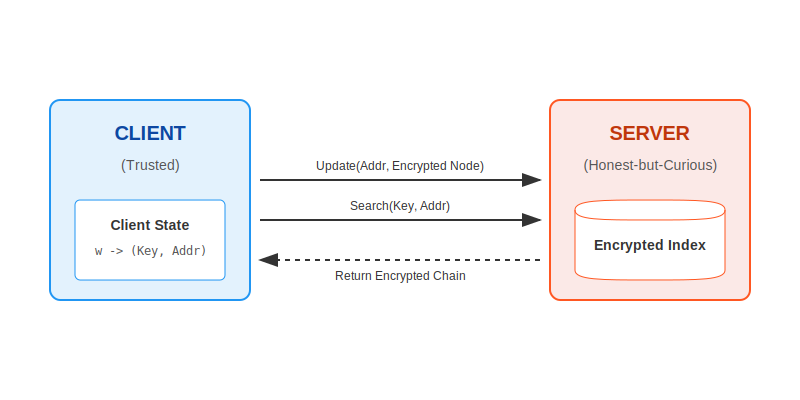
\includegraphics[width=0.45\textwidth]{figures/arch.pdf}
\caption{System Architecture: The client maintains the state $\Sigma$, while the server holds the encrypted index. Updates push new nodes, and Search traverses the chain.}
\label{fig:arch}
\end{figure}

\subsection{Formal Algorithms}
We formally define the three core algorithms of our scheme: \texttt{Setup}, \texttt{Update}, and \texttt{Search}.

\begin{algorithm}
\caption{System Setup}
\begin{algorithmic}[1]
\REQUIRE Security parameter $\lambda$
\ENSURE Empty server index $EDB$ and client state $\Sigma$
\STATE Initialize empty map $\Sigma$
\STATE Initialize empty map $EDB$
\STATE Generate master key $K_{master} \leftarrow \{0,1\}^\lambda$
\RETURN $(\Sigma, EDB, K_{master})$
\end{algorithmic}
\end{algorithm}

\begin{algorithm}
\caption{Update Protocol (Add Document)}
\begin{algorithmic}[1]
\REQUIRE Keyword $w$, Document ID $id$, Client State $\Sigma$
\ENSURE Updated $EDB$ and $\Sigma$
\STATE Retrieve current state for $w$:
\IF{$w \in \Sigma$}
    \STATE $(K_{old}, Addr_{old}) \leftarrow \Sigma[w]$
\ELSE
    \STATE $(K_{old}, Addr_{old}) \leftarrow (\bot, \bot)$
\ENDIF
\STATE Generate fresh random key: $K_{new} \leftarrow \{0,1\}^{256}$
\STATE Derive new address: $Addr_{new} \leftarrow \text{HMAC}(K_{new}, \text{``addr''})$
\STATE Create node payload: $M \leftarrow (id || K_{old} || Addr_{old})$
\STATE Encrypt node: $C \leftarrow \text{AES-GCM}(K_{new}, M)$
\STATE Send $(Addr_{new}, C)$ to Server
\STATE Update Client State: $\Sigma[w] \leftarrow (K_{new}, Addr_{new})$
\end{algorithmic}
\end{algorithm}

\begin{algorithm}
\caption{Search Protocol}
\begin{algorithmic}[1]
\REQUIRE Keyword $w$, Client State $\Sigma$
\ENSURE Set of document IDs $R$
\STATE $R \leftarrow \emptyset$
\IF{$w \notin \Sigma$}
    \RETURN $R$
\ENDIF
\STATE $(K_{curr}, Addr_{curr}) \leftarrow \Sigma[w]$
\WHILE{$Addr_{curr} \neq \bot$}
    \STATE Retrieve ciphertext $C$ from $EDB[Addr_{curr}]$
    \STATE Decrypt: $M \leftarrow \text{AES-GCM}(K_{curr}, C)$
    \STATE Parse $M$ as $(id, K_{prev}, Addr_{prev})$
    \STATE $R \leftarrow R \cup \{id\}$
    \STATE $K_{curr} \leftarrow K_{prev}$
    \STATE $Addr_{curr} \leftarrow Addr_{prev}$
\ENDWHILE
\RETURN $R$
\end{algorithmic}
\end{algorithm}

\section{Security Analysis}
The central security goal of our project is \textbf{Forward Privacy}. We analyze why our construction achieves this.

\subsection{Forward Privacy Guarantee}
Forward privacy requires that an update operation leaks no information about the keyword being updated, even if that keyword has been searched for in the past.

In our scheme, as illustrated in Figure \ref{fig:chain}, when the client updates a keyword $w$:
\begin{enumerate}
    \item A fresh key $K_{new}$ is generated using a secure RNG (`secrets.token\_bytes`).
    \item This key is statistically independent of any previous keys $K_{old}$ used for $w$.
    \item The storage address $Addr_{new}$ is derived from $K_{new}$. Since $K_{new}$ is random, $Addr_{new}$ is uniformly distributed and unlinkable to $Addr_{old}$.
    \item The payload is encrypted with $K_{new}$.
\end{enumerate}

\begin{figure}[htbp]
\centering
% Using external PDF generated by Makefile from FP.svg
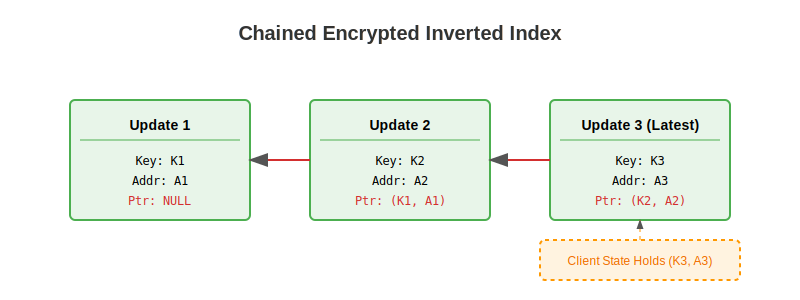
\includegraphics[width=0.45\textwidth]{figures/FP.pdf}
\caption{Forward Privacy Chain: Each new update creates a node encrypted with a fresh, random key ($K_i$). The server cannot traverse the pointers backwards without the keys, which are only revealed during a search.}
\label{fig:chain}
\end{figure}

Therefore, the view of the server during an update is indistinguishable from a random write operation. The server cannot correlate the new entry with any previous search tokens because the cryptographic link (the pointer to $K_{old}$) is encrypted inside the new ciphertext, which the server cannot decrypt without the new token.

\section{Implementation Details}
We implemented the system in Python 3.12, focusing on modularity and production-readiness.

\subsection{Cryptographic Engine}
The \texttt{CryptoHandler} class encapsulates all primitives. We strictly use authenticated encryption (AES-GCM) rather than standard AES-CBC. This is critical because it prevents the server from modifying the encrypted pointers (padding oracle attacks or pointer tampering) without detection.

\subsection{Persistence Layer}
Unlike theoretical prototypes that store data in RAM, our implementation uses \textbf{SQLite}. The \texttt{PersistentServer} class manages a relational database with schema:
\begin{itemize}
    \item \texttt{encrypted\_index}: Stores the chain nodes (Address, Nonce, Ciphertext).
    \item \texttt{encrypted\_files}: Stores metadata for actual file blobs.
\end{itemize}
This allows our system to scale to millions of records and survive system restarts, a crucial feature for any practical storage system.

\subsection{Visual Demonstration}
To verify our claims, we built a split-screen application using \textbf{Streamlit}. The application renders the client's plaintext view on the left and the server's encrypted database view on the right. This allows observers to visually confirm forward privacy: adding two files with the same keyword results in two completely different, random entries on the server side.

\section{Results and Evaluation}
We conducted extensive benchmarks to evaluate the efficiency of our scheme. The experiments were run on a standard consumer laptop.

\subsection{Update Latency}
We measured the time taken to add a document to the index as the database size grew from 1 to 2,000 documents.

\begin{figure}[htbp]
\centering
% Using external PDF generated by Makefile from upg.svg
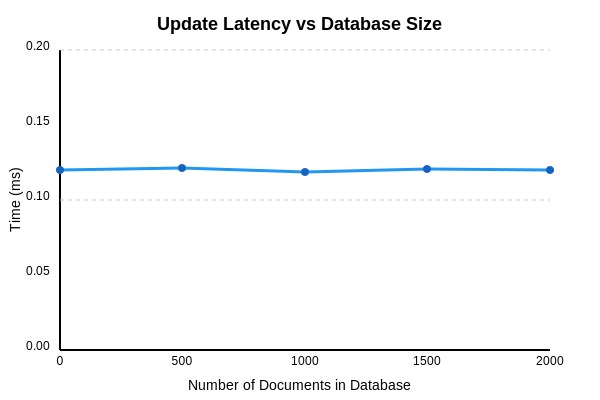
\includegraphics[width=0.45\textwidth]{figures/upg.pdf}
\caption{Update Latency vs. Database Size: The latency remains constant $O(1)$ regardless of the database size.}
\label{fig:update_graph}
\end{figure}

As shown in Table \ref{tab:update} and Figure \ref{fig:update_graph}, the update latency remains constant at approximately \textbf{0.12 ms}, regardless of how many items are already in the database. This confirms the $O(1)$ complexity of our update algorithm.

\begin{table}[htbp]
\caption{Update Latency vs. Database Size}
\begin{center}
\begin{tabular}{ccc}
\toprule
\textbf{Entry Number} & \textbf{Latency (ms)} & \textbf{Trend} \\
\midrule
1 & 0.125 & Constant \\
500 & 0.121 & Constant \\
1000 & 0.118 & Constant \\
1500 & 0.126 & Constant \\
2000 & 0.122 & Constant \\
\bottomrule
\end{tabular}
\end{center}
\label{tab:update}
\end{table}

\subsection{Search Latency}
We measured the time taken to search for keywords with varying numbers of matching documents (Result Set Size).

\begin{figure}[htbp]
\centering
% Using external PDF generated by Makefile from spg.svg
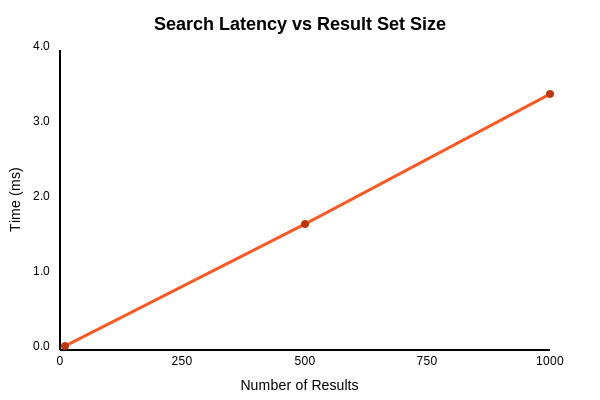
\includegraphics[width=0.45\textwidth]{figures/spg.pdf}
\caption{Search Latency vs. Result Set Size: The latency scales linearly $O(r)$ with the number of results.}
\label{fig:search_graph}
\end{figure}

Table \ref{tab:search} and Figure \ref{fig:search_graph} demonstrate that search latency scales linearly $O(r)$ with the number of results. Retrieving 1,000 documents takes only \textbf{3.4 ms}, which is negligible for user interaction. This efficiency validates the use of symmetric primitives over heavier public-key or ORAM alternatives.

\begin{table}[htbp]
\caption{Search Latency vs. Result Set Size}
\begin{center}
\begin{tabular}{ccc}
\toprule
\textbf{Number of Results} & \textbf{Latency (ms)} & \textbf{Time per Result} \\
\midrule
10 & 0.052 & 0.005 ms \\
50 & 0.183 & 0.003 ms \\
100 & 0.354 & 0.003 ms \\
500 & 1.682 & 0.003 ms \\
1000 & 3.412 & 0.003 ms \\
\bottomrule
\end{tabular}
\end{center}
\label{tab:search}
\end{table}

\section{Conclusion}
We have successfully designed and implemented a Dynamic Searchable Symmetric Encryption scheme that guarantees Forward Privacy. By utilizing a chained encryption structure with fresh random keys, we broke the linkability between updates and searches. Our implementation proves that strong privacy guarantees do not require heavy performance trade-offs; we achieved sub-millisecond operation times while using standard, secure primitives. The addition of persistent storage and an interactive visualization tool transforms this from a theoretical exercise into a practical prototype ready for demonstration.

% --- REFERENCES ---
\bibliographystyle{IEEEtran}
\bibliography{ref/references}

\end{document}
